% This file is generated by the MATLAB m-file laprint_A.m. It can be included
% into LaTeX documents using the packages graphicx and psfrag.
% It is accompanied by a postscript file. A sample LaTeX file is:
%    \documentclass{article}\usepackage{graphicx,psfrag}
%    \begin{document}% This file is generated by the MATLAB m-file laprint_A.m. It can be included
% into LaTeX documents using the packages graphicx and psfrag.
% It is accompanied by a postscript file. A sample LaTeX file is:
%    \documentclass{article}\usepackage{graphicx,psfrag}
%    \begin{document}% This file is generated by the MATLAB m-file laprint_A.m. It can be included
% into LaTeX documents using the packages graphicx and psfrag.
% It is accompanied by a postscript file. A sample LaTeX file is:
%    \documentclass{article}\usepackage{graphicx,psfrag}
%    \begin{document}% This file is generated by the MATLAB m-file laprint_A.m. It can be included
% into LaTeX documents using the packages graphicx and psfrag.
% It is accompanied by a postscript file. A sample LaTeX file is:
%    \documentclass{article}\usepackage{graphicx,psfrag}
%    \begin{document}\input{hconvergenceN1c2}\end{document}
% See http://www.mathworks.de/matlabcentral/fileexchange/loadFile.do?objectId=4638
% for recent versions of laprint.m.
%
% created by:           LaPrint version 3.16 (13.9.2004)
% created on:           08-Nov-2010 11:44:41
% eps bounding box:     15 cm x 10.4695 cm
% comment:              
%
\begin{psfrags}%
\psfragscanon%
%
% text strings:
\psfrag{s06}[t][t]{\small \setlength{\tabcolsep}{0pt}\begin{tabular}{c}h\end{tabular}}%
\psfrag{s07}[b][b]{\small \setlength{\tabcolsep}{0pt}\begin{tabular}{c}error eigenvalues\end{tabular}}%
\psfrag{s09}[b][b]{\small \setlength{\tabcolsep}{0pt}\begin{tabular}{c}h-Convergence of first nine non-zero eigenvalues for N=1 and c=0.2\end{tabular}}%
\psfrag{s10}[][]{\small \setlength{\tabcolsep}{0pt}\begin{tabular}{c} \end{tabular}}%
\psfrag{s11}[][]{\small \setlength{\tabcolsep}{0pt}\begin{tabular}{c} \end{tabular}}%
\psfrag{s12}[l][l]{\small 9}%
\psfrag{s13}[l][l]{\small 1}%
\psfrag{s14}[l][l]{\small 2}%
\psfrag{s15}[l][l]{\small 3}%
\psfrag{s16}[l][l]{\small 4}%
\psfrag{s17}[l][l]{\small 5}%
\psfrag{s18}[l][l]{\small 6}%
\psfrag{s19}[l][l]{\small 7}%
\psfrag{s20}[l][l]{\small 8}%
\psfrag{s21}[l][l]{\small 9}%
%
% xticklabels:
\psfrag{x01}[t][t]{\small $10^{0}$}%
\psfrag{x02}[t][t]{\small $10^{1}$}%
\psfrag{x03}[t][t]{\small $10^{2}$}%
%
% yticklabels:
\psfrag{v01}[r][r]{\small $10^{0}$}%
%
% Figure:
\includegraphics[width=.45\columnwidth]{hconvergenceN1c2.eps}%
\end{psfrags}%
%
% End hconvergenceN1c2.tex
\end{document}
% See http://www.mathworks.de/matlabcentral/fileexchange/loadFile.do?objectId=4638
% for recent versions of laprint.m.
%
% created by:           LaPrint version 3.16 (13.9.2004)
% created on:           08-Nov-2010 11:44:41
% eps bounding box:     15 cm x 10.4695 cm
% comment:              
%
\begin{psfrags}%
\psfragscanon%
%
% text strings:
\psfrag{s06}[t][t]{\small \setlength{\tabcolsep}{0pt}\begin{tabular}{c}h\end{tabular}}%
\psfrag{s07}[b][b]{\small \setlength{\tabcolsep}{0pt}\begin{tabular}{c}error eigenvalues\end{tabular}}%
\psfrag{s09}[b][b]{\small \setlength{\tabcolsep}{0pt}\begin{tabular}{c}h-Convergence of first nine non-zero eigenvalues for N=1 and c=0.2\end{tabular}}%
\psfrag{s10}[][]{\small \setlength{\tabcolsep}{0pt}\begin{tabular}{c} \end{tabular}}%
\psfrag{s11}[][]{\small \setlength{\tabcolsep}{0pt}\begin{tabular}{c} \end{tabular}}%
\psfrag{s12}[l][l]{\small 9}%
\psfrag{s13}[l][l]{\small 1}%
\psfrag{s14}[l][l]{\small 2}%
\psfrag{s15}[l][l]{\small 3}%
\psfrag{s16}[l][l]{\small 4}%
\psfrag{s17}[l][l]{\small 5}%
\psfrag{s18}[l][l]{\small 6}%
\psfrag{s19}[l][l]{\small 7}%
\psfrag{s20}[l][l]{\small 8}%
\psfrag{s21}[l][l]{\small 9}%
%
% xticklabels:
\psfrag{x01}[t][t]{\small $10^{0}$}%
\psfrag{x02}[t][t]{\small $10^{1}$}%
\psfrag{x03}[t][t]{\small $10^{2}$}%
%
% yticklabels:
\psfrag{v01}[r][r]{\small $10^{0}$}%
%
% Figure:
\includegraphics[width=.45\columnwidth]{hconvergenceN1c2.eps}%
\end{psfrags}%
%
% End hconvergenceN1c2.tex
\end{document}
% See http://www.mathworks.de/matlabcentral/fileexchange/loadFile.do?objectId=4638
% for recent versions of laprint.m.
%
% created by:           LaPrint version 3.16 (13.9.2004)
% created on:           08-Nov-2010 11:44:41
% eps bounding box:     15 cm x 10.4695 cm
% comment:              
%
\begin{psfrags}%
\psfragscanon%
%
% text strings:
\psfrag{s06}[t][t]{\small \setlength{\tabcolsep}{0pt}\begin{tabular}{c}h\end{tabular}}%
\psfrag{s07}[b][b]{\small \setlength{\tabcolsep}{0pt}\begin{tabular}{c}error eigenvalues\end{tabular}}%
\psfrag{s09}[b][b]{\small \setlength{\tabcolsep}{0pt}\begin{tabular}{c}h-Convergence of first nine non-zero eigenvalues for N=1 and c=0.2\end{tabular}}%
\psfrag{s10}[][]{\small \setlength{\tabcolsep}{0pt}\begin{tabular}{c} \end{tabular}}%
\psfrag{s11}[][]{\small \setlength{\tabcolsep}{0pt}\begin{tabular}{c} \end{tabular}}%
\psfrag{s12}[l][l]{\small 9}%
\psfrag{s13}[l][l]{\small 1}%
\psfrag{s14}[l][l]{\small 2}%
\psfrag{s15}[l][l]{\small 3}%
\psfrag{s16}[l][l]{\small 4}%
\psfrag{s17}[l][l]{\small 5}%
\psfrag{s18}[l][l]{\small 6}%
\psfrag{s19}[l][l]{\small 7}%
\psfrag{s20}[l][l]{\small 8}%
\psfrag{s21}[l][l]{\small 9}%
%
% xticklabels:
\psfrag{x01}[t][t]{\small $10^{0}$}%
\psfrag{x02}[t][t]{\small $10^{1}$}%
\psfrag{x03}[t][t]{\small $10^{2}$}%
%
% yticklabels:
\psfrag{v01}[r][r]{\small $10^{0}$}%
%
% Figure:
\includegraphics[width=.45\columnwidth]{hconvergenceN1c2.eps}%
\end{psfrags}%
%
% End hconvergenceN1c2.tex
\end{document}
% See http://www.mathworks.de/matlabcentral/fileexchange/loadFile.do?objectId=4638
% for recent versions of laprint.m.
%
% created by:           LaPrint version 3.16 (13.9.2004)
% created on:           08-Nov-2010 11:44:41
% eps bounding box:     15 cm x 10.4695 cm
% comment:              
%
\begin{psfrags}%
\psfragscanon%
%
% text strings:
\psfrag{s06}[t][t]{\small \setlength{\tabcolsep}{0pt}\begin{tabular}{c}h\end{tabular}}%
\psfrag{s07}[b][b]{\small \setlength{\tabcolsep}{0pt}\begin{tabular}{c}error eigenvalues\end{tabular}}%
\psfrag{s09}[b][b]{\small \setlength{\tabcolsep}{0pt}\begin{tabular}{c}h-Convergence of first nine non-zero eigenvalues for N=1 and c=0.2\end{tabular}}%
\psfrag{s10}[][]{\small \setlength{\tabcolsep}{0pt}\begin{tabular}{c} \end{tabular}}%
\psfrag{s11}[][]{\small \setlength{\tabcolsep}{0pt}\begin{tabular}{c} \end{tabular}}%
\psfrag{s12}[l][l]{\small 9}%
\psfrag{s13}[l][l]{\small 1}%
\psfrag{s14}[l][l]{\small 2}%
\psfrag{s15}[l][l]{\small 3}%
\psfrag{s16}[l][l]{\small 4}%
\psfrag{s17}[l][l]{\small 5}%
\psfrag{s18}[l][l]{\small 6}%
\psfrag{s19}[l][l]{\small 7}%
\psfrag{s20}[l][l]{\small 8}%
\psfrag{s21}[l][l]{\small 9}%
%
% xticklabels:
\psfrag{x01}[t][t]{\small $10^{0}$}%
\psfrag{x02}[t][t]{\small $10^{1}$}%
\psfrag{x03}[t][t]{\small $10^{2}$}%
%
% yticklabels:
\psfrag{v01}[r][r]{\small $10^{0}$}%
%
% Figure:
\includegraphics[width=.45\columnwidth]{hconvergenceN1c2.eps}%
\end{psfrags}%
%
% End hconvergenceN1c2.tex
